\begin{center}
    \Huge{\textbf{\underline{Chapter 1: Introduction}}}
\end{center}

\setcounter{section}{0}

\vspace{0.35cm}


\section{Compiler Definition}

\begin{prettyBox}{What's a Compiler?}{myblue}
A compiler is a software program that takes a piece of code as input, analyzes
it for errors, and generates output in the form of messages or logs.
Additionally, it produces an executable file that can be run on a computer.
\end{prettyBox}

\vspace{0.25cm}
\section{Steps of Compilation}
\begin{prettyBox}{Steps}{myblue}
The process of compilation is done following these steps chronologically:
\begin{enumerate}
    \item Lexical Analysis
    \item Syntactic Analysis (Parsing)
    \item Semantic Analysis
        \begin{itemize}
            \item Generation of Intermediate Code
            \item Syntax-Directed Translation
        \end{itemize}
    \item Generation of Object Code
\end{enumerate}
\end{prettyBox}

\vspace{0.25cm}

\subsection{Lexical Analysis}
\begin{prettyBox}{Lexical Analysis}{myblue}
Lexical analysis consists of dividing the entire code into lexical entities (tokens) and evaluating each of them independently. Tokens can be divided based on:
\begin{itemize}
    \item Spaces
    \item Logical operators (AND, OR, NOT, \(>\)=, \(>\), \(<\)=, \(<\), =)
    \item Arithmetic operators (+, -, *, /)
    \item Separators ([ ], \{ \}, ( ))
\end{itemize}
\end{prettyBox}

\newpage
\underline{\textbf{Example}}

\begin{center}
    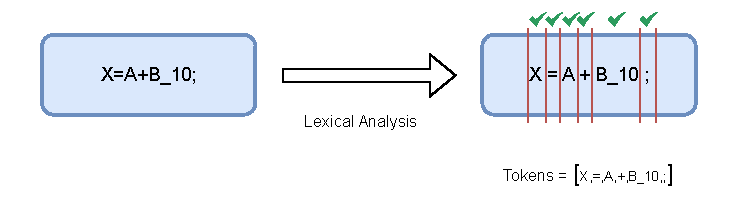
\includegraphics{Chapters/Examples/Intro/ex1.drawio.pdf}
\end{center}

\vspace{0.25cm}
\begin{center}
    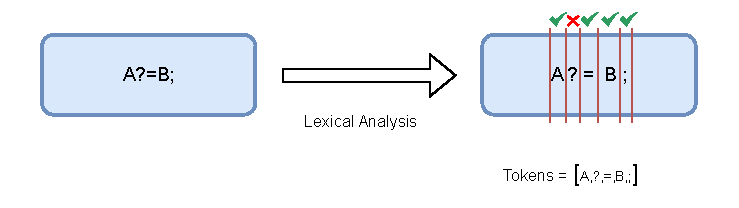
\includegraphics{Chapters/Examples/Intro/ex2.drawio.pdf}
\end{center}

\vspace{0.35cm}


\subsection{Syntactic Analysis (Parsing)}
\begin{prettyBox}{Syntactic Analysis}{myblue}
Syntactic analysis checks if the order of tokens is correct and adheres to the required format (using automata or regular expressions).  
There are two methods:  
\begin{itemize}
    \item Descending methods  
    \item Ascending methods  
\end{itemize}
\end{prettyBox}

\vspace{0.95cm}
\underline{\textbf{Example}}

\vspace{0.35cm}
\begin{center}
    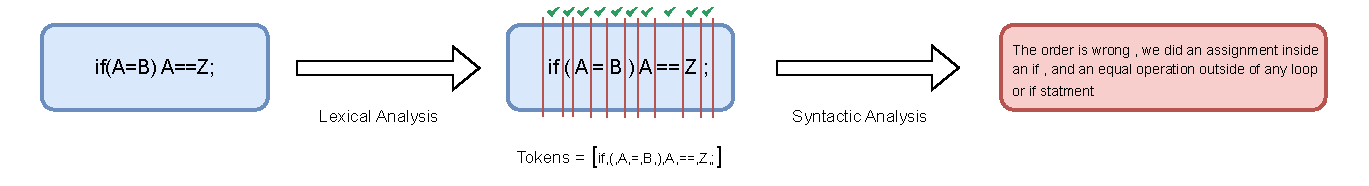
\includegraphics[height=0.17\textheight,width=0.9\textwidth]{Chapters/Examples/Intro/ex3.drawio.pdf}
\end{center}

\newpage

\begin{prettyBox}{Note}{red}
If a code is lexically correct, it does not guarantee that it will be syntactically correct. However, the opposite is true:

\begin{center}
    Correct Syntactically $\rightarrow$ Correct Lexically \\[0.15cm]
    Correct Lexically $\nrightarrow$ Correct Syntactically
\end{center}

\end{prettyBox}

\vspace{0.35cm}

\subsection{Semantic Analysis}
\begin{prettyBox}{Semantic Analysis}{myblue}
This phase ensures the code is logically correct and adheres to the language's rules. It verifies \textbf{type mismatches, variable declarations, function calls, and more}.

\begin{itemize}
    \item \textbf{Generation of Intermediate Code}: 
    Produces a simplified, platform-independent representation of the program. This step is crucial for optimizing the code and converting it into machine code later.
    \begin{itemize}
        \item \textbf{Quadruple Form}
        \item \textbf{Postfix and Prefix Forms}
    \end{itemize}

    \item \textbf{Syntax-Directed Translation}: 
    Generates intermediate representations, ensuring that the semantics (meaning) of the program guide the creation of subsequent steps.
\end{itemize}
\end{prettyBox}

\vspace{0.35cm}
\subsection{Object Code Generation}

\begin{prettyBox}{Object Code Generation}{myblue}
The final step of compilation, where the object code is generated to execute the program.
This is the only step in the compilation process that we will not cover in this course.
\end{prettyBox}

\vspace{1cm}
\section{Compilation Steps Diagram}

\vspace{0.3cm}
\begin{center}
    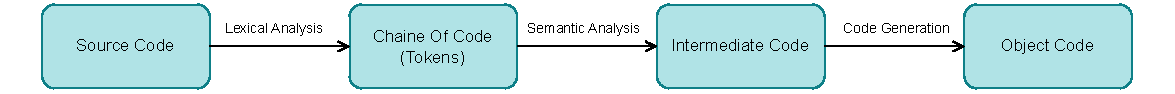
\includegraphics[height=0.08\textheight]{Chapters/Examples/Intro/sum.drawio.pdf}
\end{center}




